\section{Introduction}
\label{sec:intro}

Raman spectroscopy is a widely used, non-destructive analytical technique for probing the vibrational fingerprints of inorganic materials. In mineralogical and solid-state chemical analysis, Raman spectra provide information on local bonding environments, anionic groups, lattice vibrations, hydration states, and structural disorder, making them useful for differentiating chemically related inorganic families such as silicates, oxides, carbonates, sulfates, phosphates, sulfides, halides, and borates \cite{farmer1974minerals,mcmillan1984ramanglasses,nakamoto2009infraredraman,lafuente2015rruff}. X-ray diffraction (XRD), in contrast, provides crystallographic and phase-level information through diffraction-peak positions and intensities. The combination of Raman spectroscopy and XRD therefore offers complementary vibrational and structural evidence for inorganic material characterization, phase screening, and mineral identification \cite{grazulis2009cod,grazulis2012cod,guo2024xrddeeplearning,rincon2025simpod,guo2024pxrdnet}.

Despite the availability of open spectral and crystallographic resources, converting raw instrument outputs into reproducible machine-learning-ready datasets remains challenging. Raw Raman and XRD files can contain nonuniform wavenumber or $2\theta$ axes, missing or invalid rows, duplicate spectral points, baseline drift caused by fluorescence or background scattering, instrumental noise, and arbitrary intensity scaling. These issues make direct comparison across spectra difficult and can degrade downstream classification or property-prediction models if not handled systematically \cite{savitzky1964smoothing,zhang2010airpls,baek2015arpls,rinnan2009preprocessing}. For inorganic materials, the problem is further complicated by polymorphism, mixed phases, hydration, compositional substitutions, and overlapping vibrational bands, all of which can cause chemically meaningful spectral variation within the same broad material family.

Machine learning has become an important tool in materials informatics, enabling rapid screening of chemical composition, crystal structures, and materials properties from high-dimensional descriptors and database-derived representations \cite{jain2013materialsproject,ward2018matminer,choudhary2020jarvis,dunn2020matbench,riebesell2025matbenchdiscovery}. Recent work has also demonstrated the usefulness of ML for Raman spectral analysis, mineral classification, and diffraction-based phase or structure prediction \cite{dai2024libsraman,eranti2026ramanencoder,zhang2026physramannet,liu2026ramanclassificationreview,li2024pxrdgen,guo2024xrddeeplearning}. However, many existing studies either rely on task-specific or proprietary datasets, use preprocessed spectra without exposing the raw-file-to-model pipeline, focus on a single modality, or provide limited chemical interpretation of the learned decision process. Consequently, there remains a need for an open, reproducible Raman--XRD benchmark that connects raw spectral files, inorganic chemical-family labels, materials-property annotations, and confidence-aware screening outputs.

To address this gap, we introduce \textbf{Spec2Prop-InorgBench}, a curated open-data Raman--XRD benchmark for AI-assisted inorganic materials screening. The benchmark integrates open Raman and XRD spectral resources with formula-normalized inorganic family labels and materials-property annotations. Beyond dataset construction, we develop a runtime preprocessing workflow that parses raw spectral files, removes invalid entries, sorts and deduplicates spectral axes, interpolates spectra to a fixed representation, corrects baseline effects, smooths spectral noise, and normalizes intensities before feature extraction. This design explicitly bridges the gap between raw instrumental output and deployable machine-learning inference.

The proposed screening workflow, \textbf{Spec2Prop-Edge}, uses chemistry-aware spectral descriptors together with efficient machine-learning models for preliminary inorganic material-family prediction. In particular, the deployment-oriented classifier is based on LightGBM-DART, a gradient-boosted decision-tree framework suitable for heterogeneous tabular features and small-to-moderate spectral datasets \cite{ke2017lightgbm,rashmi2015dart}. We further extend the workflow to spectra-to-property prediction for band-gap class, metal/non-metal classification, and formation-energy class, linking spectral information with materials-informatics labels \cite{xie2018cgcnn,chen2019megnet,goodall2020roost,wang2021crabnet,choudhary2021alignn}. The aim is not to replace expert spectroscopic interpretation or crystallographic validation, but to provide a confidence-aware screening assistant that can prioritize candidate material families and guide further laboratory verification.

The main contributions of this work are summarized as follows:
\begin{itemize}
\item We construct \textbf{Spec2Prop-InorgBench}, an open Raman--XRD inorganic spectral benchmark linking Raman spectra, optional XRD patterns, inorganic family labels, and materials-property annotations.
\item We develop a runtime Raman/XRD preprocessing pipeline that converts raw spectral files into standardized model-ready representations.
\item We design chemistry-aware spectral descriptors that combine global spectral-shape information with peak, band-window, moment, and prototype-similarity features.
\item We evaluate machine-learning models for nine-class inorganic family screening under leakage-safe validation and report confidence-aware top-$k$ performance.
\item We extend the benchmark to spectra-to-property prediction for band-gap, metallicity, and formation-energy classes.
\item We demonstrate \textbf{Spec2Prop-Edge} as a deployment-style screening workflow for preliminary material-family interpretation and candidate prioritization.
\end{itemize}

\begin{figure}[!ht]
\centering
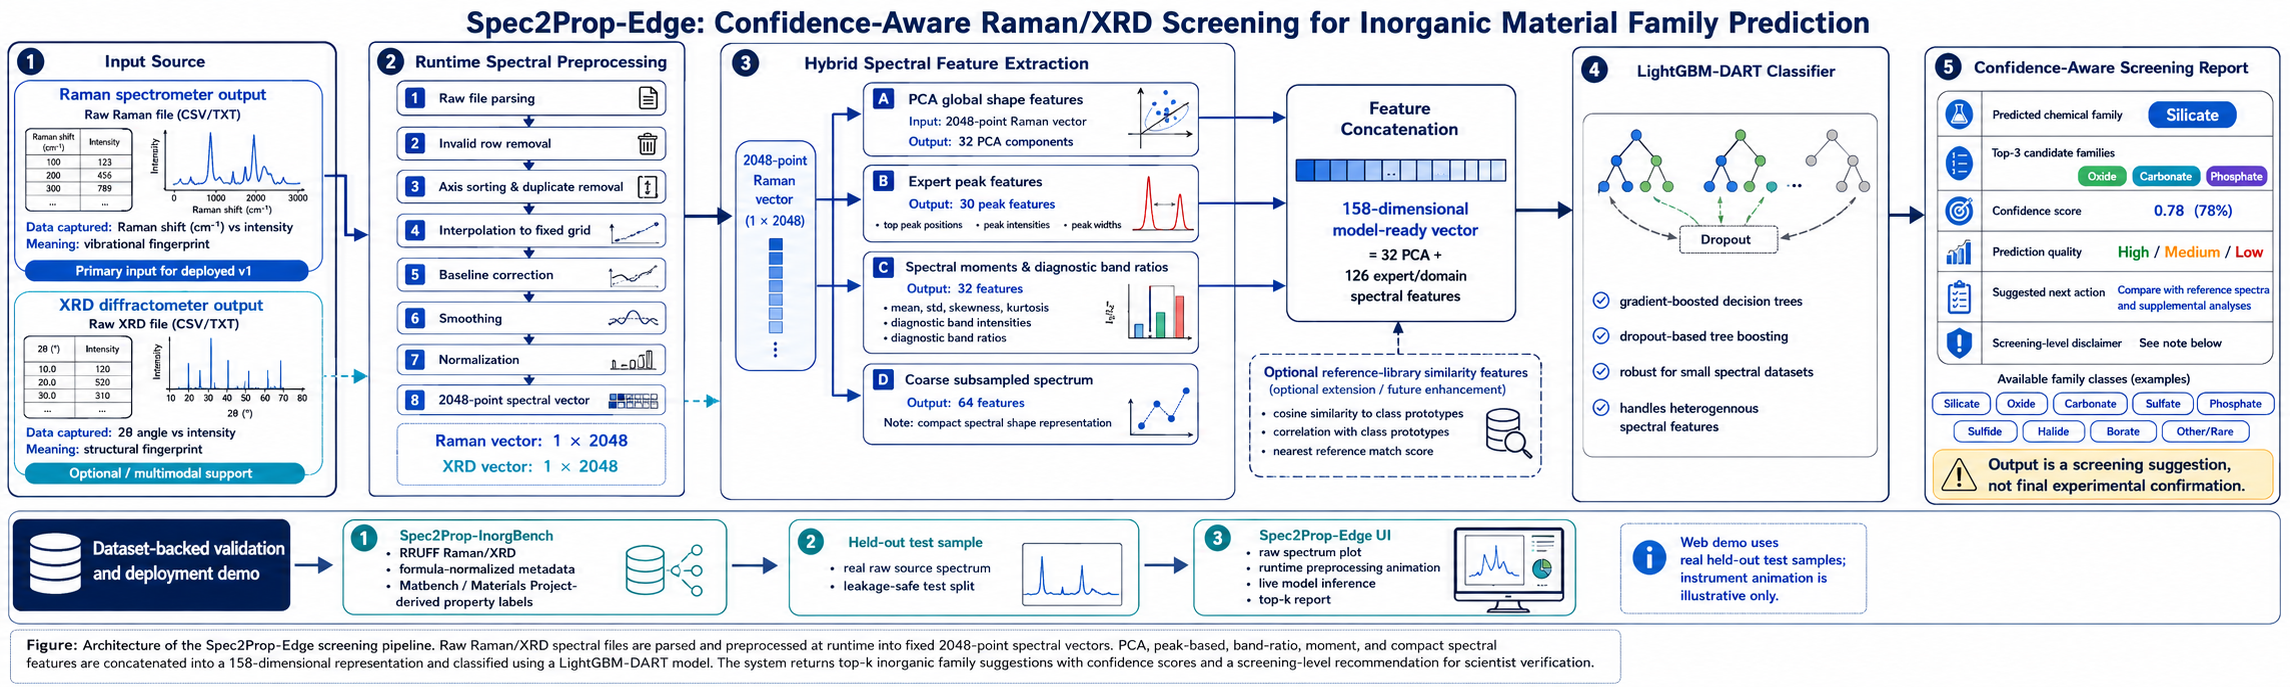
\includegraphics[width=\linewidth]{figures/pipeline.png}
\caption{Overall workflow of Spec2Prop-InorgBench and Spec2Prop-Edge. Open Raman and XRD spectral resources are curated, formula-normalized, linked with inorganic family and materials-property labels, transformed into model-ready spectral representations, and used for confidence-aware inorganic material screening.}
\label{fig:workflow}
\end{figure}

The remainder of this manuscript is organized as follows. Section~\ref{sec:methods} describes the data sources, dataset construction, spectral preprocessing, feature extraction, machine-learning models, and leakage-safe evaluation protocol. Section~\ref{sec:results} presents the inorganic family-screening results, spectra-to-property prediction results, Raman--XRD multimodal analysis, and chemical interpretation of model features. Section~\ref{sec:limitations} discusses the current limitations and future directions, and Section~\ref{sec:conclusion} concludes the paper.
